\documentclass[12pt, notitlepage]{article}

\usepackage{fullpage}
\usepackage{listings}
\usepackage{color}
\usepackage{graphicx}

\definecolor{gray}{rgb}{0.5,0.5,0.5}
\definecolor{dkgreen}{rgb}{0,0.6,0}
\definecolor{mauve}{rgb}{0.58,0,0.82}

\lstset{
backgroundcolor=\color{white},
frame=single,
title=\lstname, 
keywordstyle=\color{blue}, 
commentstyle=\color{dkgreen}, 
stringstyle=\color{mauve},
showspaces=false,               
showstringspaces=false
}

\begin{document}



\title{Habitat Simulation}
\author{Abel Souza, Derek Weitzel, Douglas Silva}
\date{December 7, 2012}

\maketitle

\section{Introduction}

\section{Implementation}


\subsection{Replacing random number nenerator}

\section{Evaluation}

In order to evaluate the habitat parallelization, we created input parameters that would span possible parameters used by researchers in the simulation.  The application has two main parameters, the landscape size and the number of starting agents.  Since we parallelized the execution of agents, we expect that the application will scale well with the number of agents.  Also, a larger landscape can handle more agents.  We created input parameter files that included different landscape dimensions and starting agents, as shown in Table \ref{tab:parameters}.

\begin{table}[ht]
\centering
\begin{tabular}{ c | c }
\textbf{Dimensions} & \textbf{Starting Agents} \\ 
\hline \hline
129 x 129 & 300 \\
129 x 129 & 800 \\
200 x 200 & 5000 \\
500 x 500 & 800 \\
500 x 500 & 50000 \\
1024 x 1024 & 1000
\end{tabular}
\caption{Input parameters} \label{tab:parameters}
\end{table}

The habitat executable opens the files \texttt{habitat.in} and \texttt{makeland.in} when it begins execution.  \texttt{habitat.in} contains both the dimensions of the landscape and the number of starting agents.  \texttt{makeland.in} only includes the dimensions of the landscape.

Evaluation jobs where submitted to Tusker with the submission script shown in Listing \ref{lst:submissionfile}.

\begin{figure}[ht]
\centering
\lstinputlisting[language=bash,title=pbs.sh,caption={Submission file used for evaluation},label={lst:submissionfile}]{Include/pbs.sh}
\end{figure}

As you can see from the submit script in Listing \ref{lst:submissionfile}, the habitat runs execute in isolation.  First it creates a temporary directory and copies the input files and habitat executable into the temporary directory.  Next it starts the execution and times it.  The stderr of the job includes the job run time.  For the purposes of timing, we use the \texttt{real} time output.

The parameters in Table \ref{tab:parameters} where executed at 7 different core counts: 1, 2, 4, 8, 16, 32, 48.  At each core count, we ran 30 identical jobs to get a good sampling.  For analysis, we averaged the 30 runs at each parameter and core count.  Therefore there where over $7 * 6 * 30 = 1260$ runs.  There where also several re-runs, and a previous set of runs before replacing the random number generator, totaling over 2100 runs of the habitat simulation.

\subsection{Results}

The first set of results are runtimes for one of the runs.

\begin{table}[ht]
\centering
\begin{tabular}{ r | r }
\textbf{Cores} & \textbf{Runtime (m)} \\
\hline \hline
1 & 186.81\\
2 & 142.89\\
4 & 85.59\\
8 & 61.23\\
16 & 37.11\\
32 & 29.49\\
48 & 26.16\\
\end{tabular}
\caption{Runtimes for 1024 x 1024 and 1000 starting agents} \label{tab:runtimes}
\end{table}

1024 x 1024 is a very large landscape for Drew.  He is unable to run a landscape this large on his own machine due to the memory requirements.

\begin{figure}[ht]
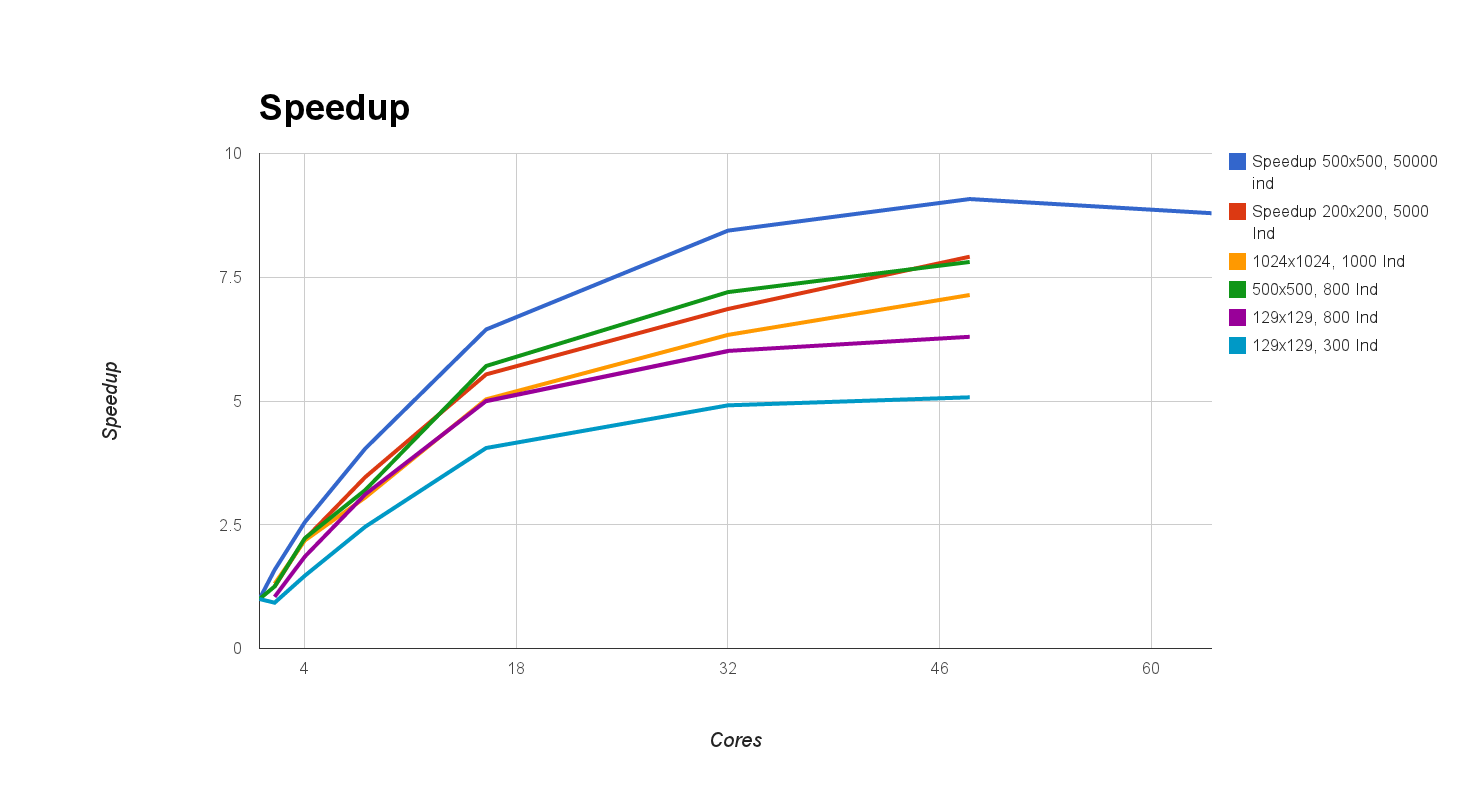
\includegraphics[width=\textwidth]{Include/SpeedupRuns.png}
\caption{Speedup for all Runs} \label{fig:speedup}
\end{figure}


Speedup is shown in Figure \ref{fig:speedup}.  The speedup plateaus for all runs around 32 or 48 cores.  Next we look at efficiency of, shown in Figure \ref{fig:efficiency}.  The efficiency also drops off significantly as the core count increases.

\begin{figure}[ht]
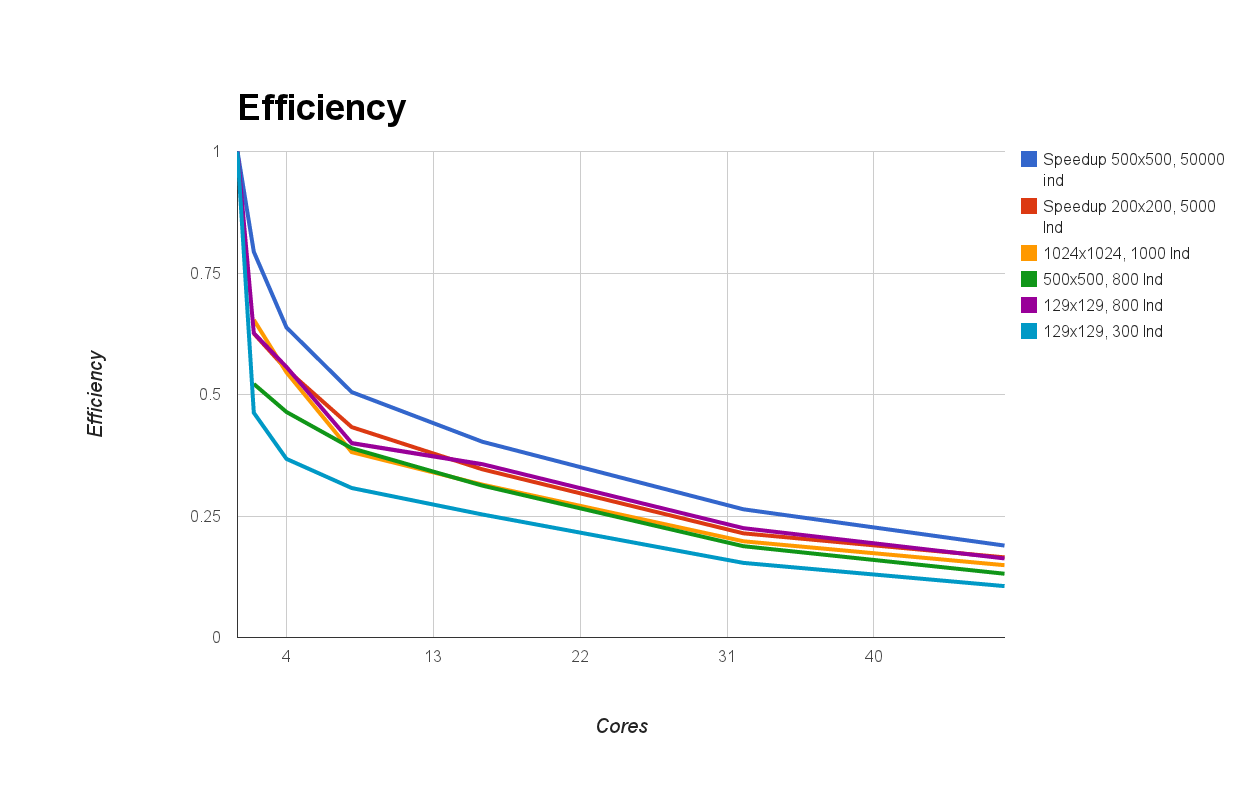
\includegraphics[width=\textwidth]{Include/Efficiency.png}
\caption{Efficiency for all Runs} \label{fig:efficiency}
\end{figure}


Both the efficiency and speedup graphs show that application only scales well to around 32 cores.  To verify that this matches with the expected scalability of the application, we have to first look at the call graph.  The original call graph is shown in Figure \ref{fig:originalcall}.

\begin{figure}[ht]
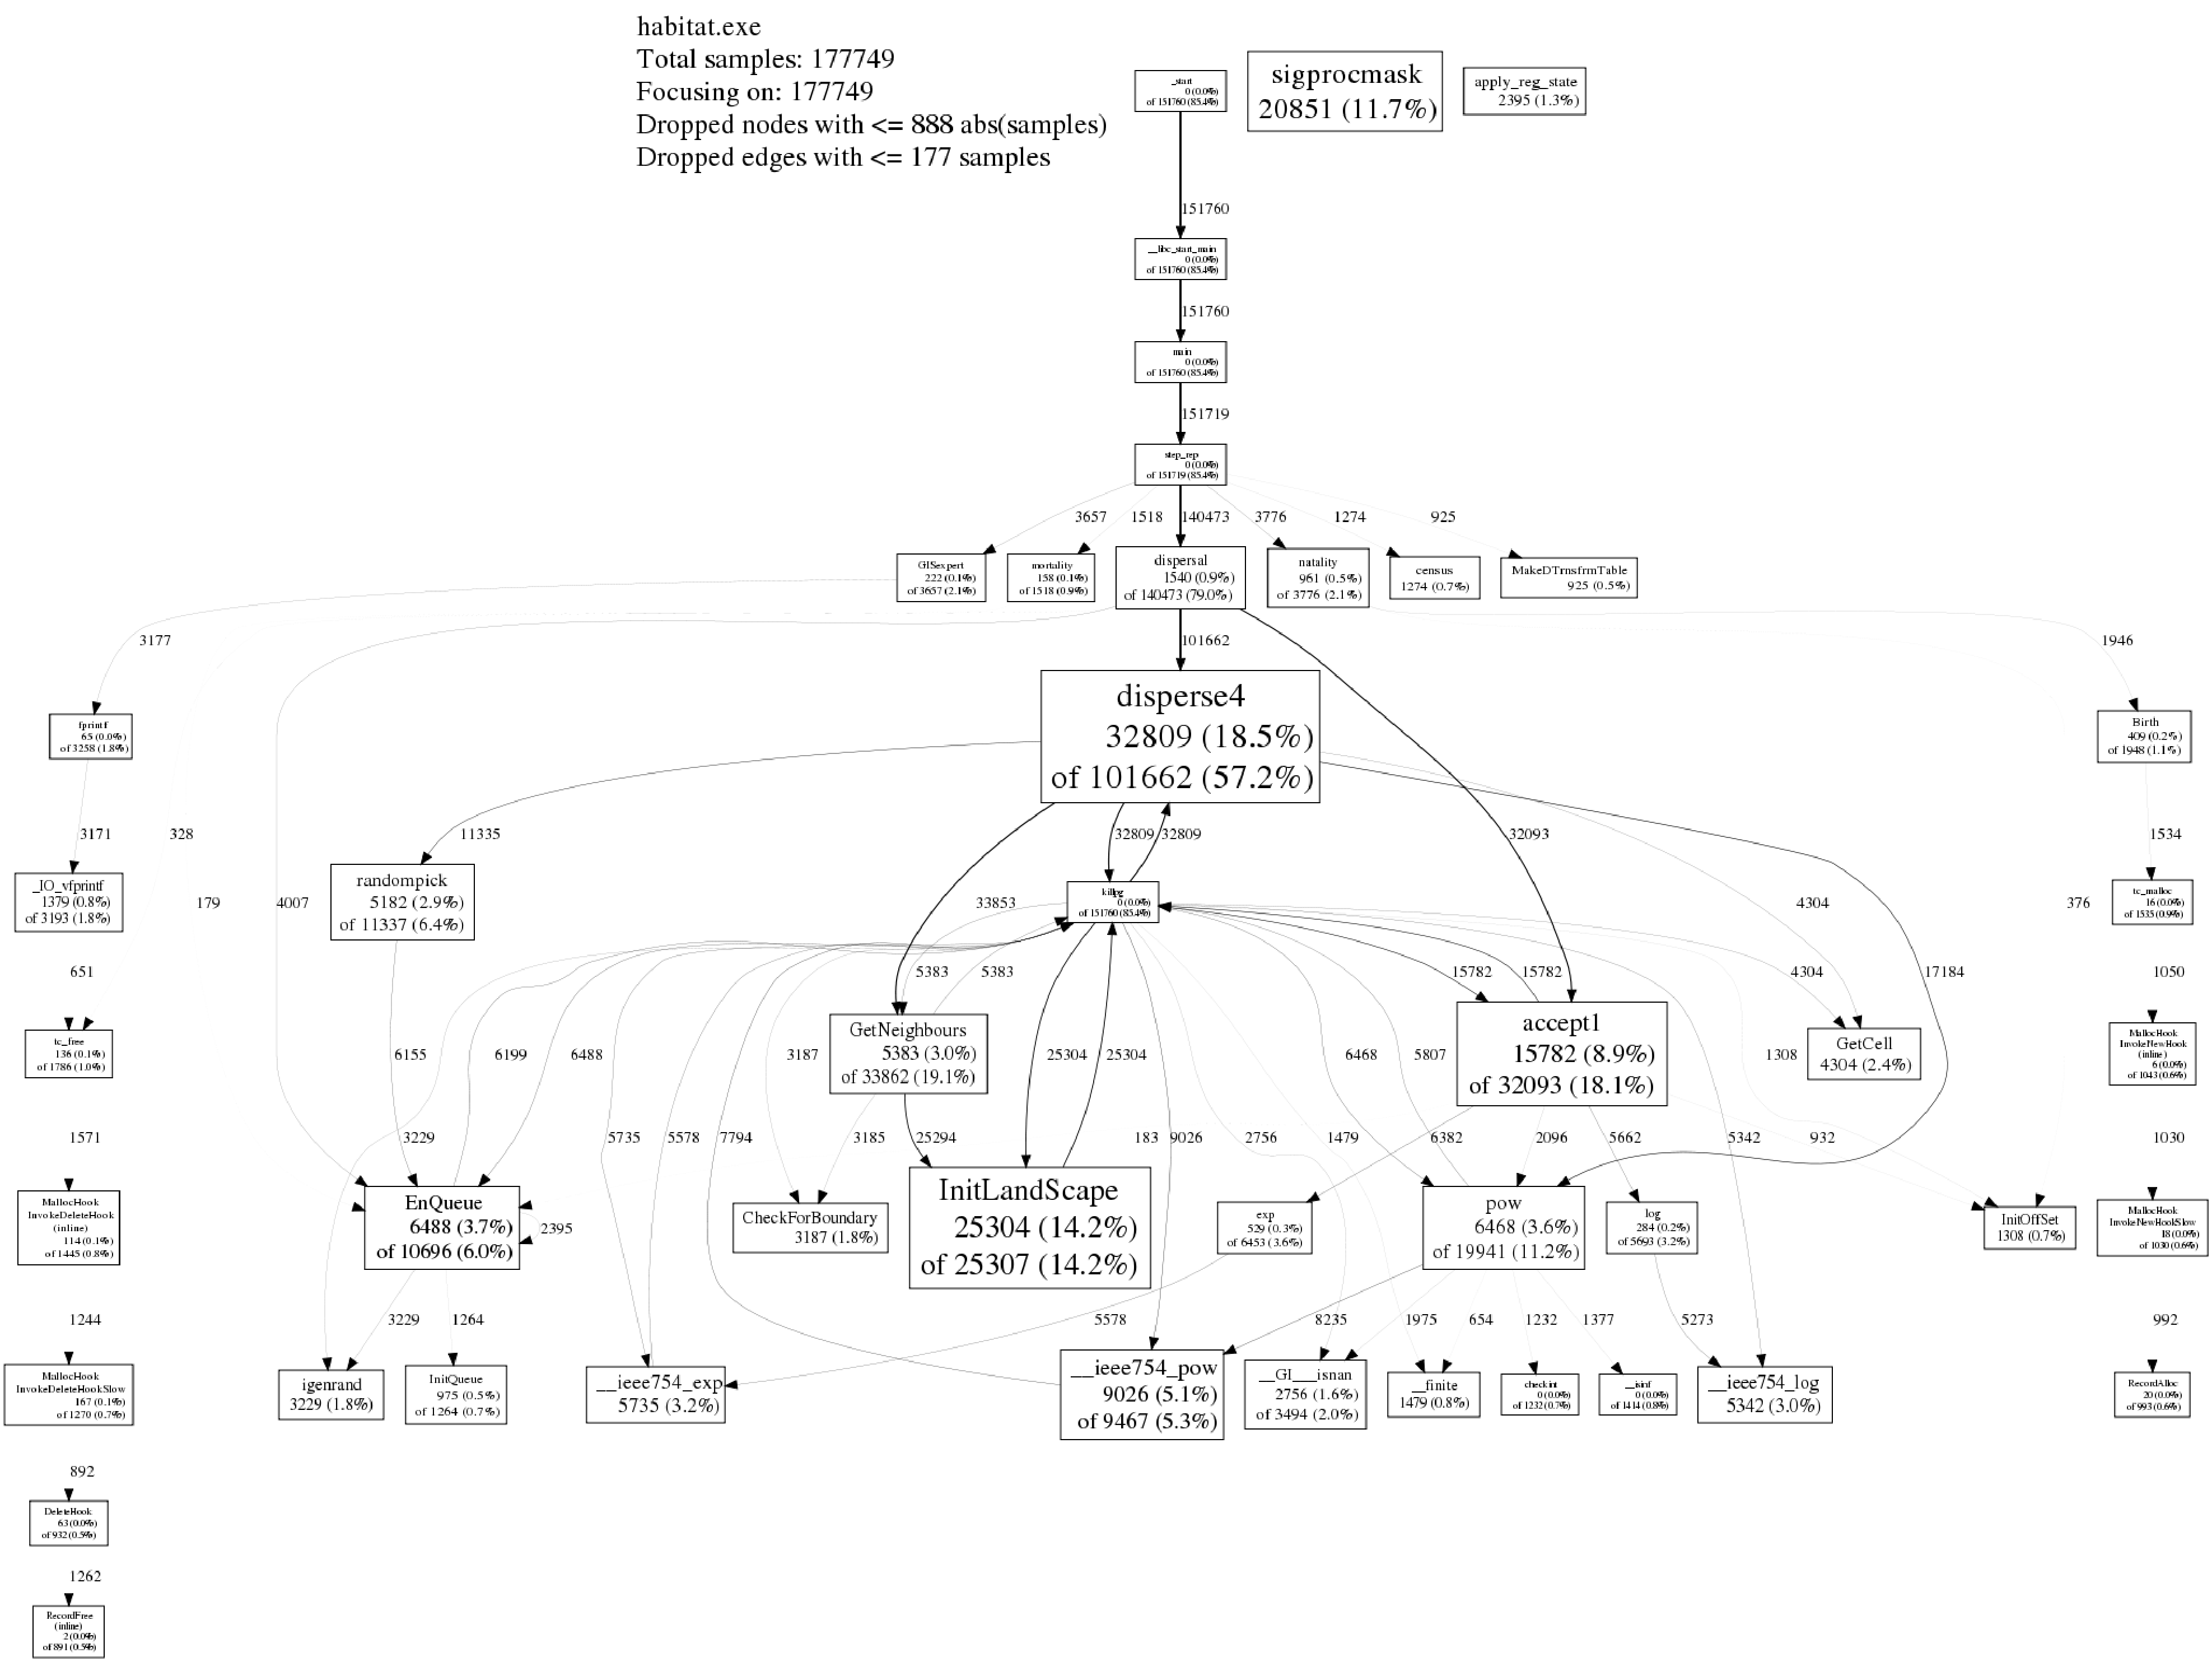
\includegraphics[width=\textwidth]{Include/originalcall.pdf}
\caption{Call graph for the non-parallelized habitat simulation} \label{fig:originalcall}
\end{figure}


As you can see in Figure \ref{fig:originalcall}, The parallelized function is \texttt{dispersal}, which callee's takes about 79.0\% of the execution time.  Putting 79\% into Amdahl's law, we can compare the theorized speedup with the actual.  The comparison is shown in Figure \ref{fig:amdahls}.  As you can see, the expected and the actual speedups match nearly in the shape and magnitude.  

\begin{figure}[ht]
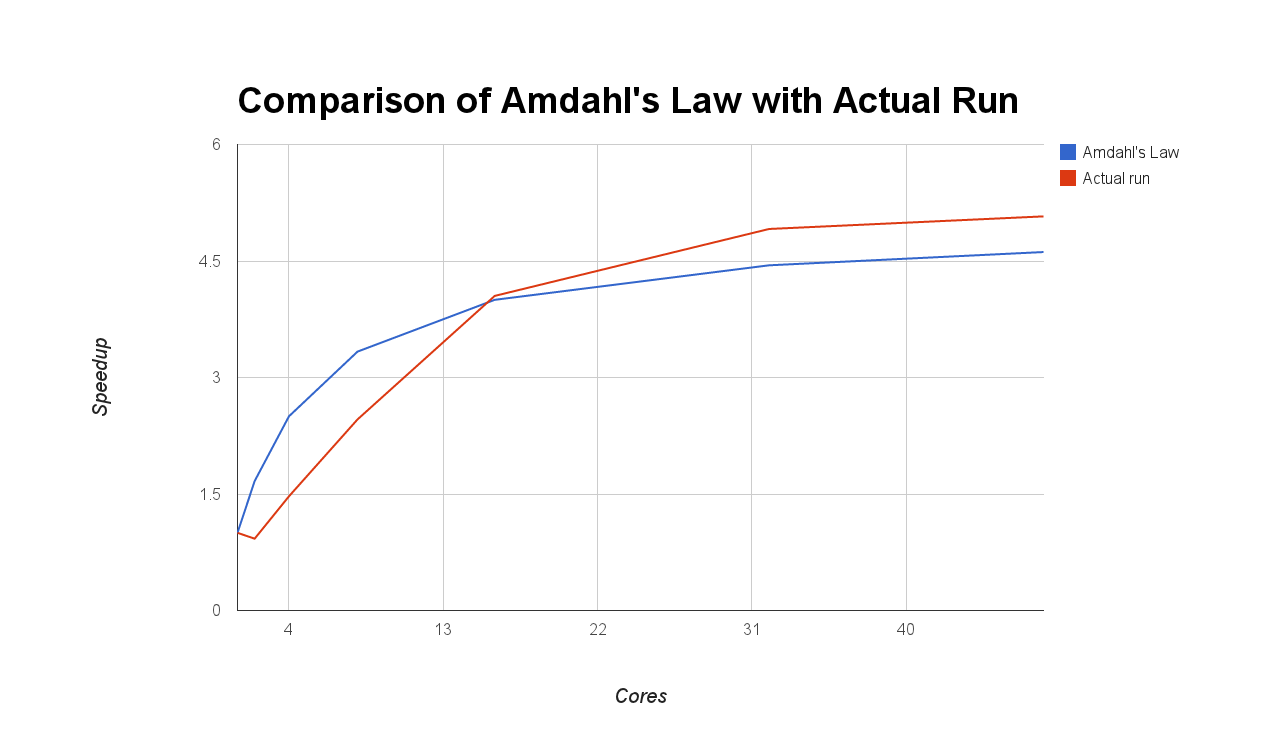
\includegraphics[width=\textwidth]{Include/amdahls.png}
\caption{Comparison of Amdahl's theorized speedup at 79\%} \label{fig:amdahls}
\end{figure}

The parallel call graph is shown in Figure \ref{fig:parallelcall}.  You can see that \texttt{omp_get_num_procs} function is taking a large amount of the processing time.  We could not determine why it is taking so much time, but you can see that it is being called by the OpenMP lock and unlock functions.

\section{Conclusions}

\end{document}